\chapter{L1 Trigger Pre-Firing}
\label{sec:prefire}

When an L1 seed is triggered to accept an event (\emph{L1A}), the following two bunch crossings (not necessarily corresponding to collisions) are blocked from firing L1As. 
At most, two in four consecutive events can fire L1A (i.e. the sequence L1A, blocked, blocked, L1A).
Figure~\ref{fig:vbf:pre1} is an example of a normal ECAL L1 seed accepting an event and blocking the subsequent bunch crossings.
In what follows, we will refer to the bunch crossing with an interesting collision (i.e. the one we would like the trigger to select) as \bx{0}.

\begin{figure}
    \begin{center}
        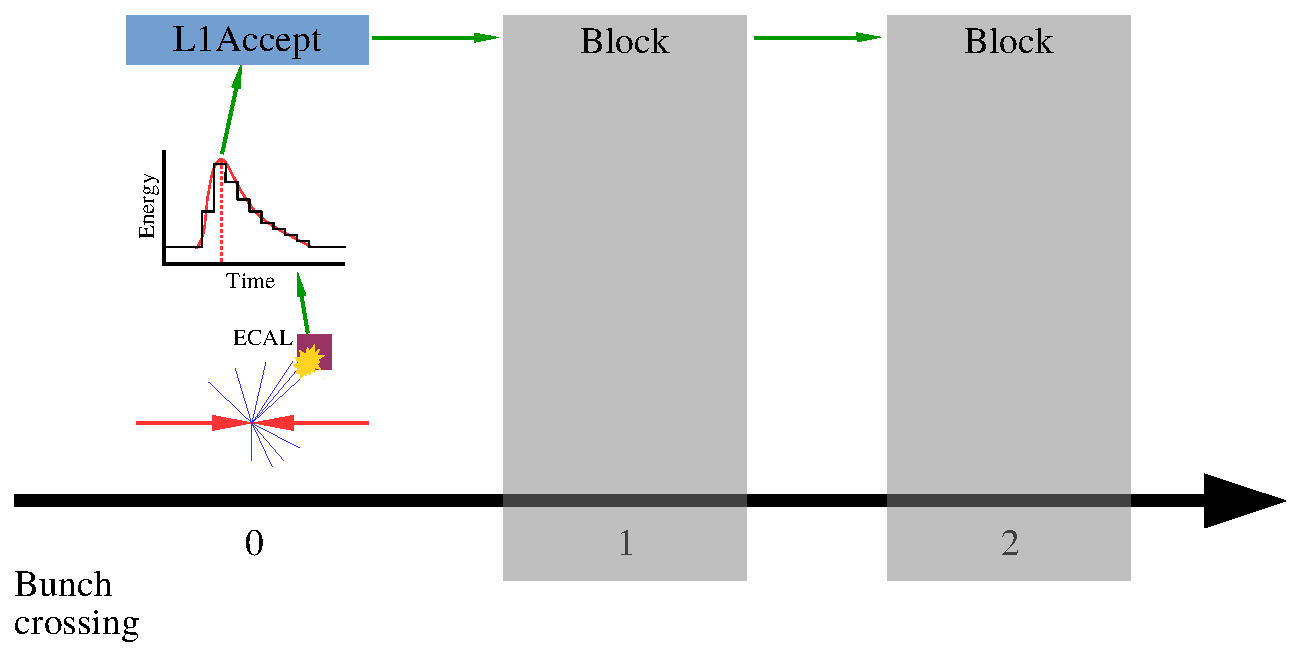
\includegraphics[width=0.8\textwidth,page=1]{figures/vbf/triggers/l1diag.pdf}
        \caption{A normal event in which an ECAL seed triggers the L1A signal. 
                 The subsequent two bunch crossings are blocked. 
                 \bx{0}~refers to the event containing the physics object of interest.
                 Green arrows indicate causality.}
        \label{fig:vbf:pre1}
    \end{center}
\end{figure}

A pre-fire refers to the case in which a malformed detector signal is mis-reconstructed, so that the peak of the pulse appears to have occurred in the previous bunch crossing (\bx{-1}).   
In this particular case, a region of the ECAL ($2.5 < |\eta|<3$) suffered from a loss in transparency due to radiation damage and would produce pulse shapes that are poorly described by the model used to extract the pulse energy and time. 
When this happens, the L1 seeds for ECAL-based signatures (e.g. electron triggers) can fire an L1A for \bx{-1}.
This ECAL L1 seed in \bx{-1}~will set to zero the corresponding ECAL clusters in \bx{0} (known as zero suppression), further biasing the event description.
So, we would have an L1A for an arbitrary event (\bx{-1}), and the interesting event (\bx{0}) would be blocked from passing the L1 altogether. 
This is depicted in Figure~\ref{fig:vbf:pre2}.
Typically, \bx{-1}~contains uninteresting physics signatures, and so is not accepted by the HLT.

\begin{figure}
    \begin{center}
        \includegraphics[width=0.8\textwidth,page=2]{figures/vbf/triggers/l1diag.pdf}
        \caption{A pre-fired event in which an ECAL seed triggers the L1A signal for \bx{-1}. 
                 The subsequent two bunch crossings (including the one of interest) are blocked. 
                 \bx{0}~refers to the event containing the physics object of interest.
                 Green arrows indicate causality.}
        \label{fig:vbf:pre2}
    \end{center}
\end{figure}

To measure how often an ECAL energy deposit (typically left by a jet) causes an event to be lost by pre-firing, we need to compute the following efficiency:
\begin{equation}
    \epsilon_\text{pre-fire}(\pt,\eta,\phi) = \frac{N_\text{pre-fire}(\pt,\eta,\phi)}{N_\text{all events}(\pt,\eta,\phi)}
\end{equation}
However, by definition, pre-fired events cannot be recorded, and therefore $N_\text{pre-fire}(\pt,\eta,\phi)$ is difficult to measure.
A very small subset of the recorded dataset ($0.2\%$) consists of \emph{un-pre-fireable} events.
These are recorded events (\bx{0}) in which an L1A fired 3 bunch crossings prior (\bx{-3}).
Due to the blocking rules, L1A cannot fire in \bx{-2}~and \bx{-1}.
Even if there is an ECAL seed in \bx{0}~that pre-fires, it will be blocked from firing an L1A, and therefore \bx{0}~is protected.
If some other object in \bx{0}~manages to pass L1 and HLT decisions, then \bx{0}~will be recorded and can be studied.
A schematic of such events is shown in Figure~\ref{fig:vbf:pre3}.

\begin{figure}
    \begin{center}
        \includegraphics[width=0.8\textwidth,page=3]{figures/vbf/triggers/l1diag.pdf}
        \caption{An un-pre-fireable event in which \bx{-3}~protects \bx{0}~from being pre-fired. 
                 Green arrows indicate causality.}
        \label{fig:vbf:pre3}
    \end{center}
\end{figure}

The L1 trigger system records trigger primitive (TP) information (4-vectors of physics objects considered in an L1 selection) for \bx{-1}~if \bx{0}~is triggered.
This means we can identify the cases in which a physics object in \bx{0}~coincides with a TP in \bx{-1}, indicating a pre-fire. 
Therefore (using the bunch crossing numbering in Figure~\ref{fig:vbf:pre3}), we re-define the efficiency:
\begin{equation}
    \epsilon_\text{pre-fire}(\pt,\eta,\phi) = \frac{N_\text{pre-fire \bx{0}|\bx{-3}}(\pt,\eta,\phi)}{N_\text{\bx{0}|\bx{-3}}(\pt,\eta,\phi)}
\end{equation}
By definition, all events in this ratio will be recorded. 
Figure~\ref{fig:vbf:pre_eff2_etaphi} shows this efficiency as a function of jet location. 
We observe there is a \emph{hot} ECAL tower near the location $\eta=-2.8$ and $\phi=2$.
Not only does this tower fire very frequently (leading to many particles, leading to many jets), but it almost always pre-fires.
To first order, events with a jet in this crystal should be rejected.
Beyond this, there is very little localization in the pre-fire probability (besides restriction to the ECAL endcap). 

\begin{figure}[]
    \begin{center}
        \begin{subfigure}[t]{0.49\textwidth}
            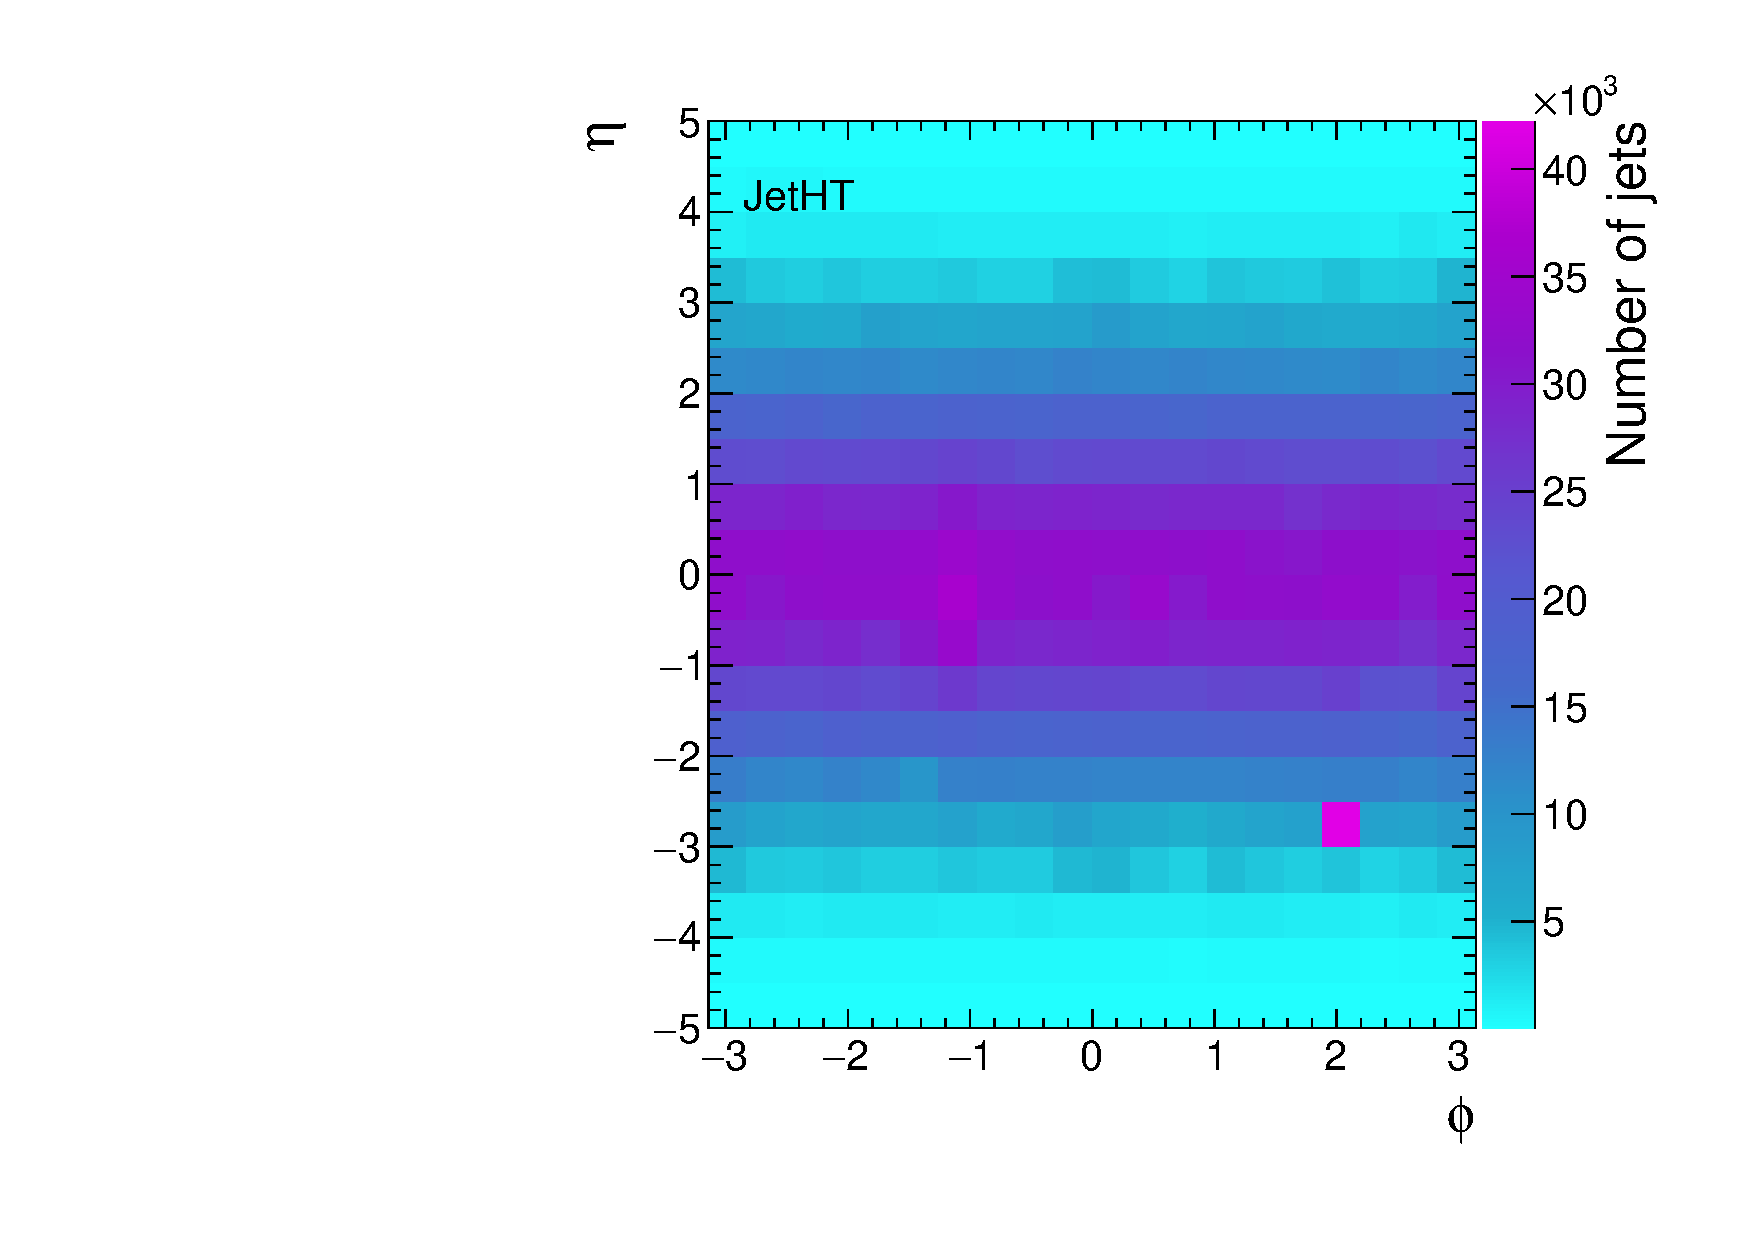
\includegraphics[width=\textwidth]{figures/vbf/triggers/JetHT_inclusive_egiso_etaphi_den.pdf}
            \caption{Number of jets}
        \end{subfigure}
        \begin{subfigure}[t]{0.49\textwidth}
            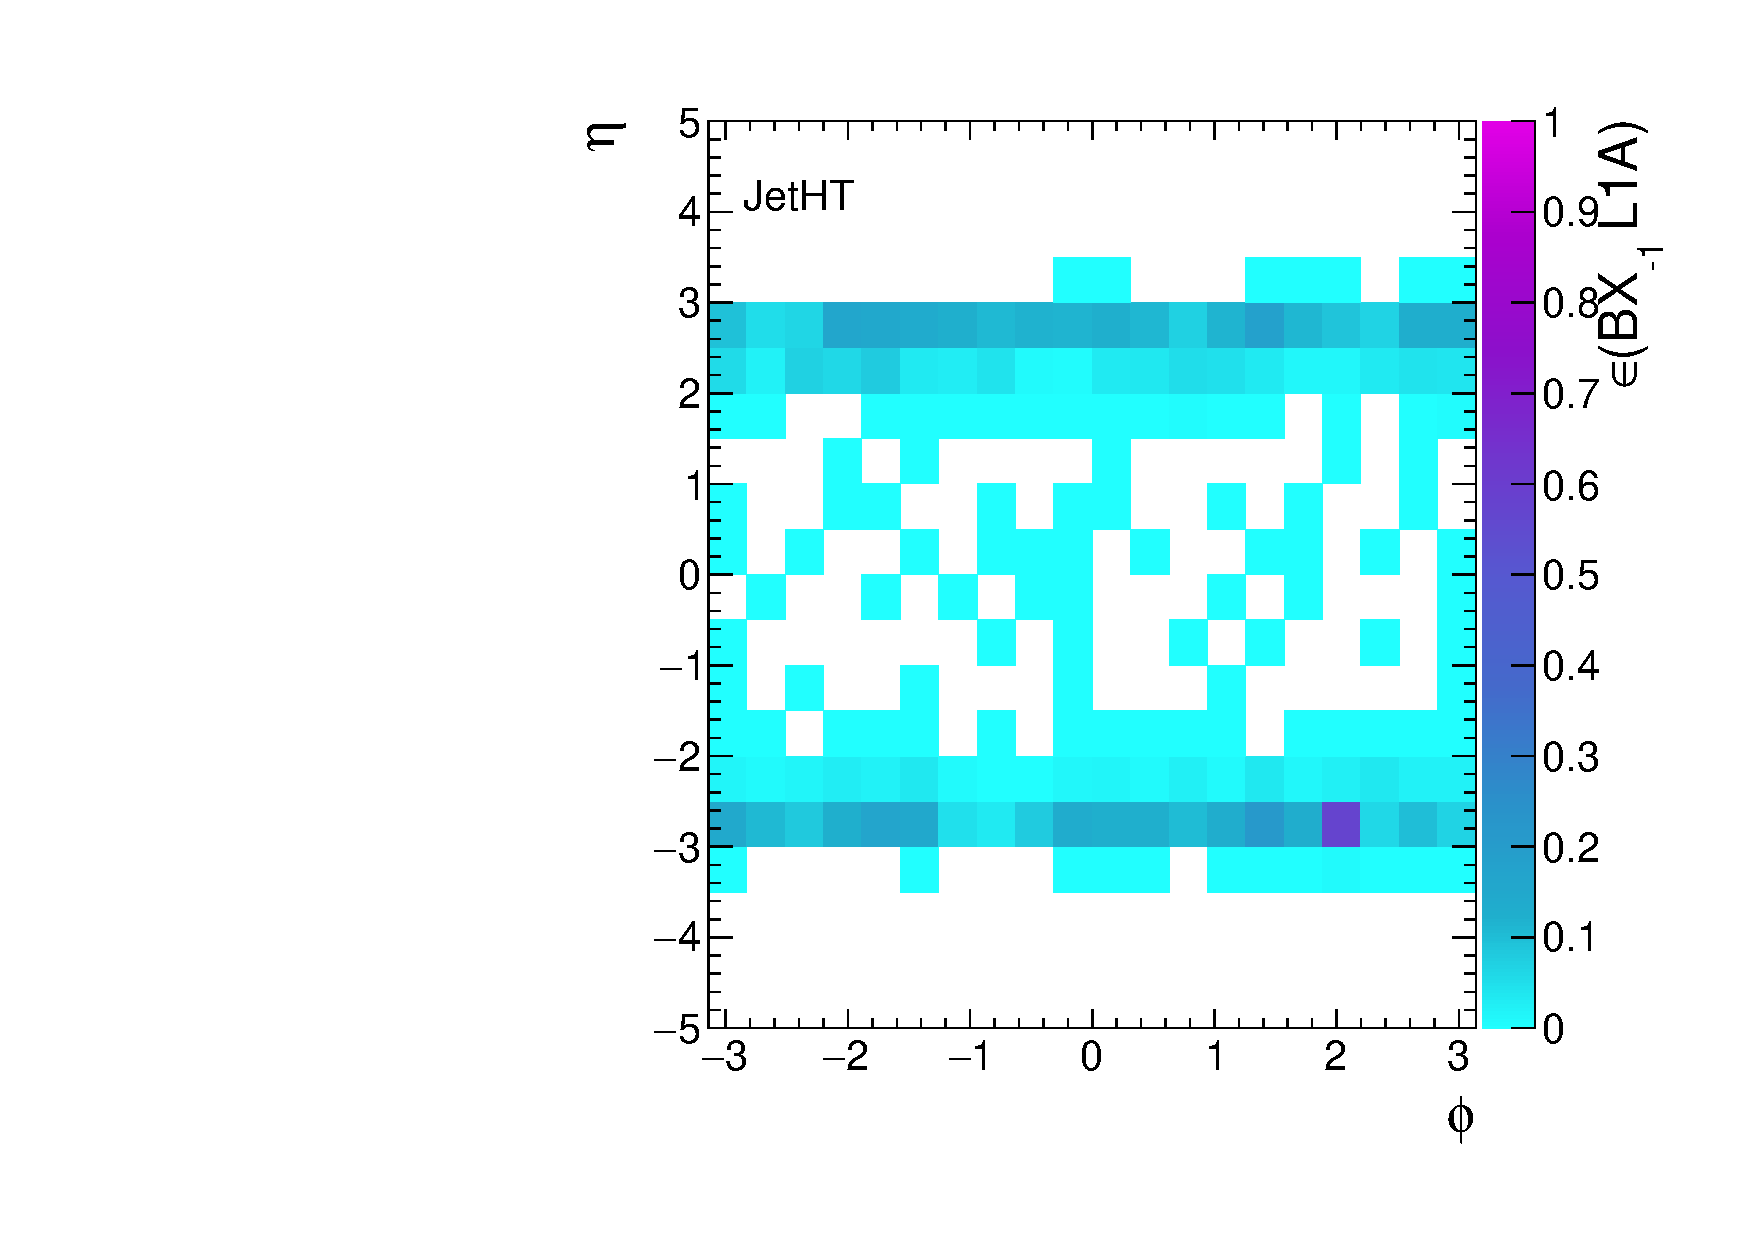
\includegraphics[width=\textwidth]{figures/vbf/triggers/JetHT_inclusive_egiso_etaphi_ratio.pdf}
            \caption{Pre-fire probability}
        \end{subfigure}
        \caption{Distribution of jets and pre-fire events as a function of the jet location in the detector.
                 Note the spike near $(\eta,\phi) = (-2.8,2)$. }
        \label{fig:vbf:pre_eff2_etaphi}
    \end{center}
\end{figure}

In Figure~\ref{fig:vbf:pre_eff1} we see $\epsilon_\text{pre-fire}$ as a function of $\pt$ in a restricted $\eta$ range.
Firstly, we observe that $\epsilon_\text{pre-fire}$ increases as a function of $\pt$, and the turn-on is sharper as a function of EM $\pt$. 
This is explained by the mechanism of the pre-fire: the individual ECAL trigger seeds have a threshold of 30 GeV.
The higher the jet $\pt$, the higher the probability of the jet depositing $30$ GeV of EM energy in a localized area, setting off an L1 seed. 
Secondly, we observe a strong dependence on the reference triggers used to select $\bx{0}$.
For example, jet-based triggers (JetHT) lead to a much higher efficiency than $\ptmiss$-based triggers (MET).  
This is a consequence of zero suppression biasing the \bx{0}~triggers, as shown diagrammatically in Figure~\ref{fig:vbf:pre_diag}.
Muon-based triggers (SingleMuon) are largely unaffected by the ECAL system, and therefore this measurement of $\epsilon_\text{pre-fire}$ is the least biased.  

\begin{figure}[]
    \begin{center}
        \begin{subfigure}[t]{0.49\textwidth}
            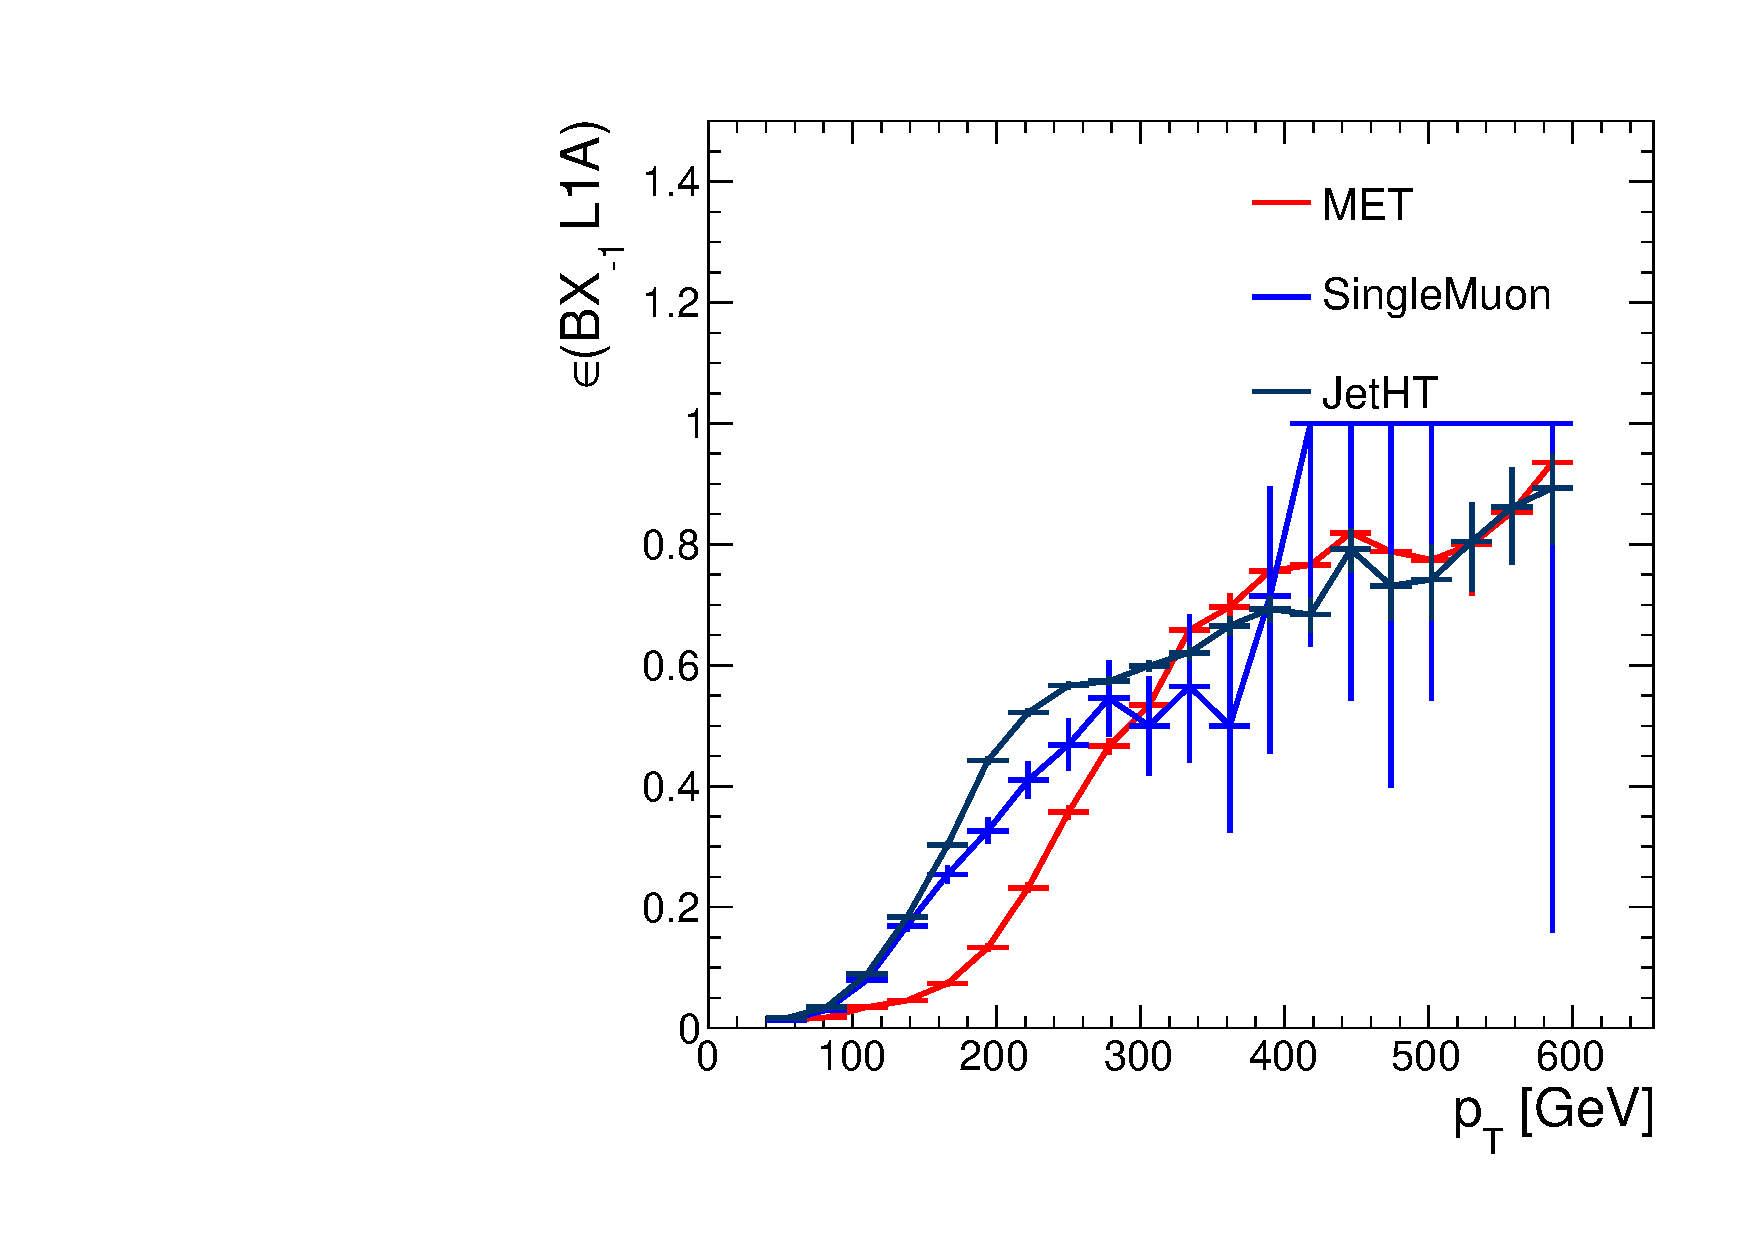
\includegraphics[width=\textwidth]{figures/vbf/triggers/oned_jotPt_finor_ratio.pdf}
            \caption{$\pt$}
        \end{subfigure}
        \begin{subfigure}[t]{0.49\textwidth}
            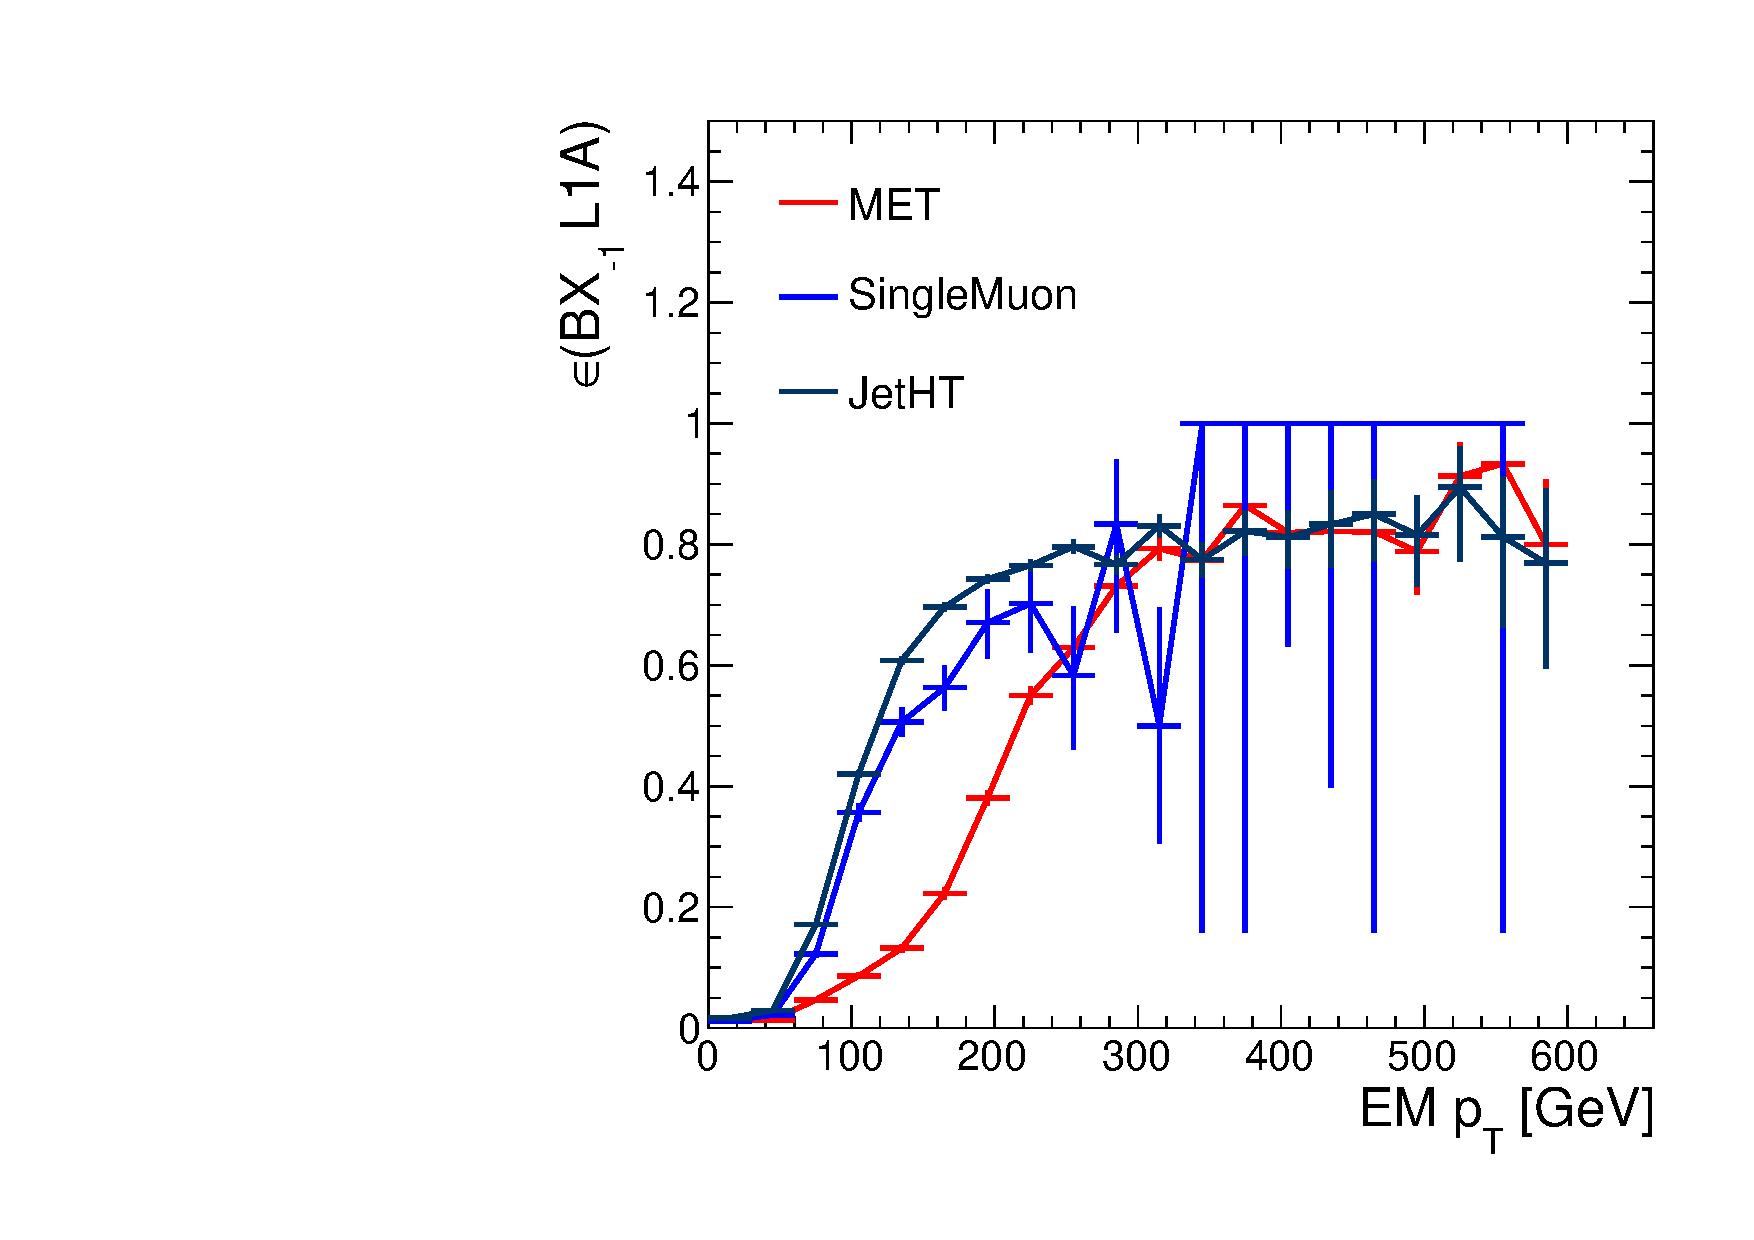
\includegraphics[width=\textwidth]{figures/vbf/triggers/oned_jotEMPt_finor_ratio.pdf}
            \caption{$\pt \times E_\mathrm{ECAL}/E_\mathrm{total}$}
        \end{subfigure}
        \caption{Probability that a given jet with $2.25<|\eta|<3$ causes a pre-fire in the L1 trigger due to ECAL mistiming.
                 Two parameterizations are used: jet $\pt$ and EM $\pt$.
                 The three curves refer to which set of triggers are used to select $\bx{0}$.}
        \label{fig:vbf:pre_eff1}
    \end{center}
\end{figure}

\begin{figure}[]
    \begin{center}
        \begin{subfigure}[t]{0.49\textwidth}
            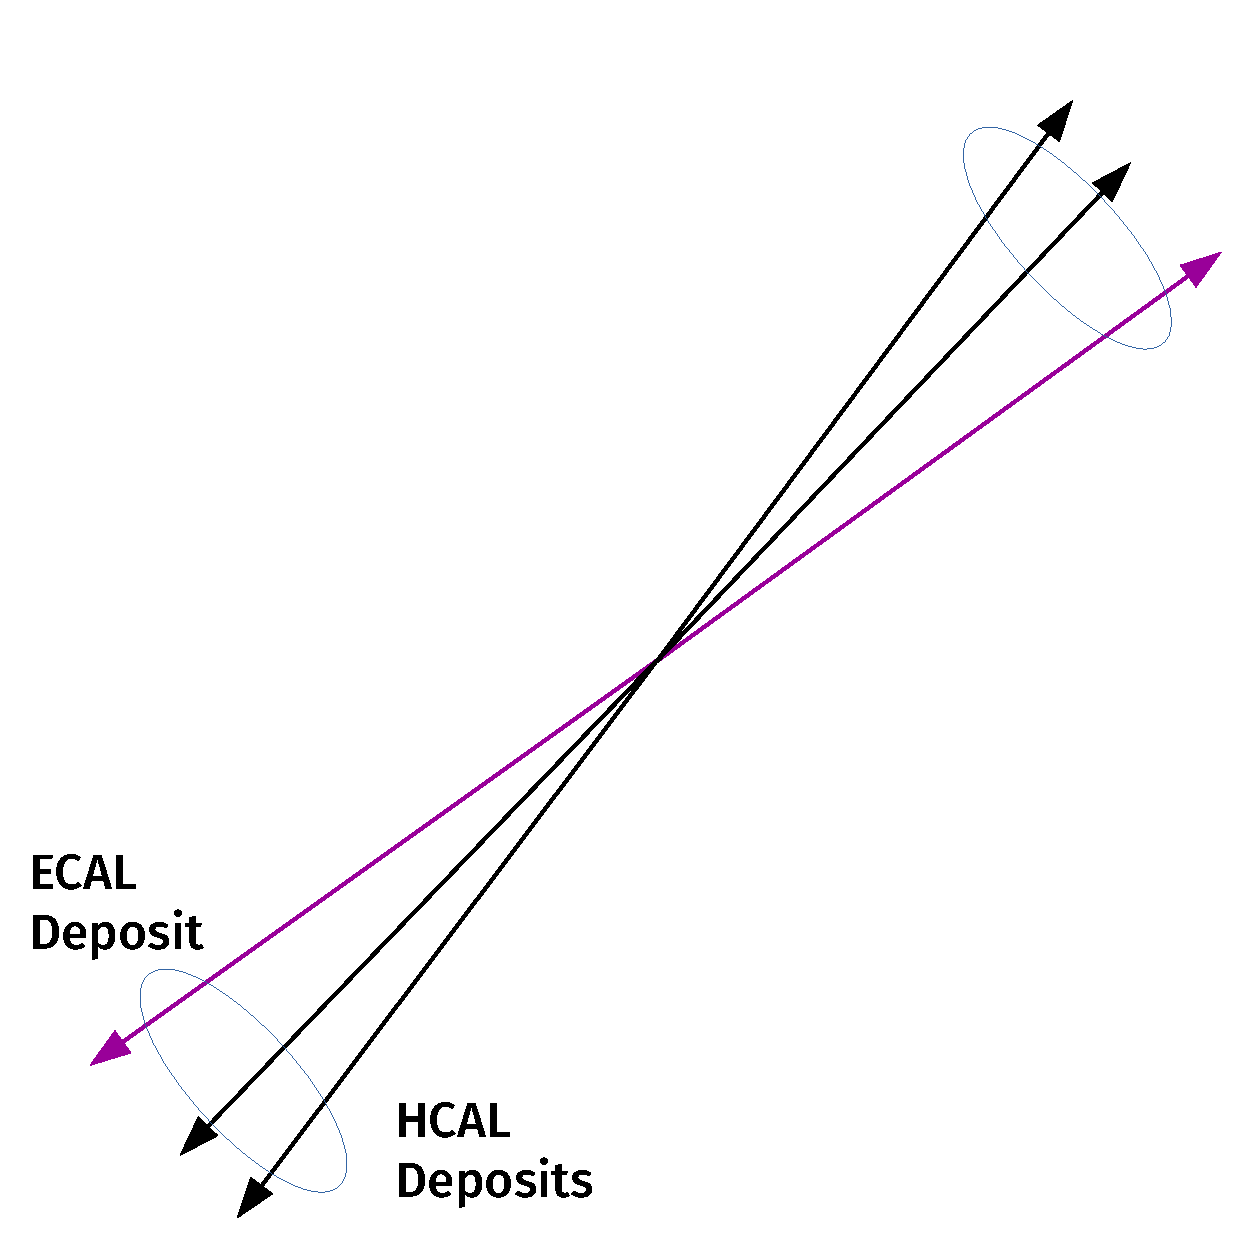
\includegraphics[width=0.49\textwidth]{figures/vbf/triggers/normal_dijet.pdf}
            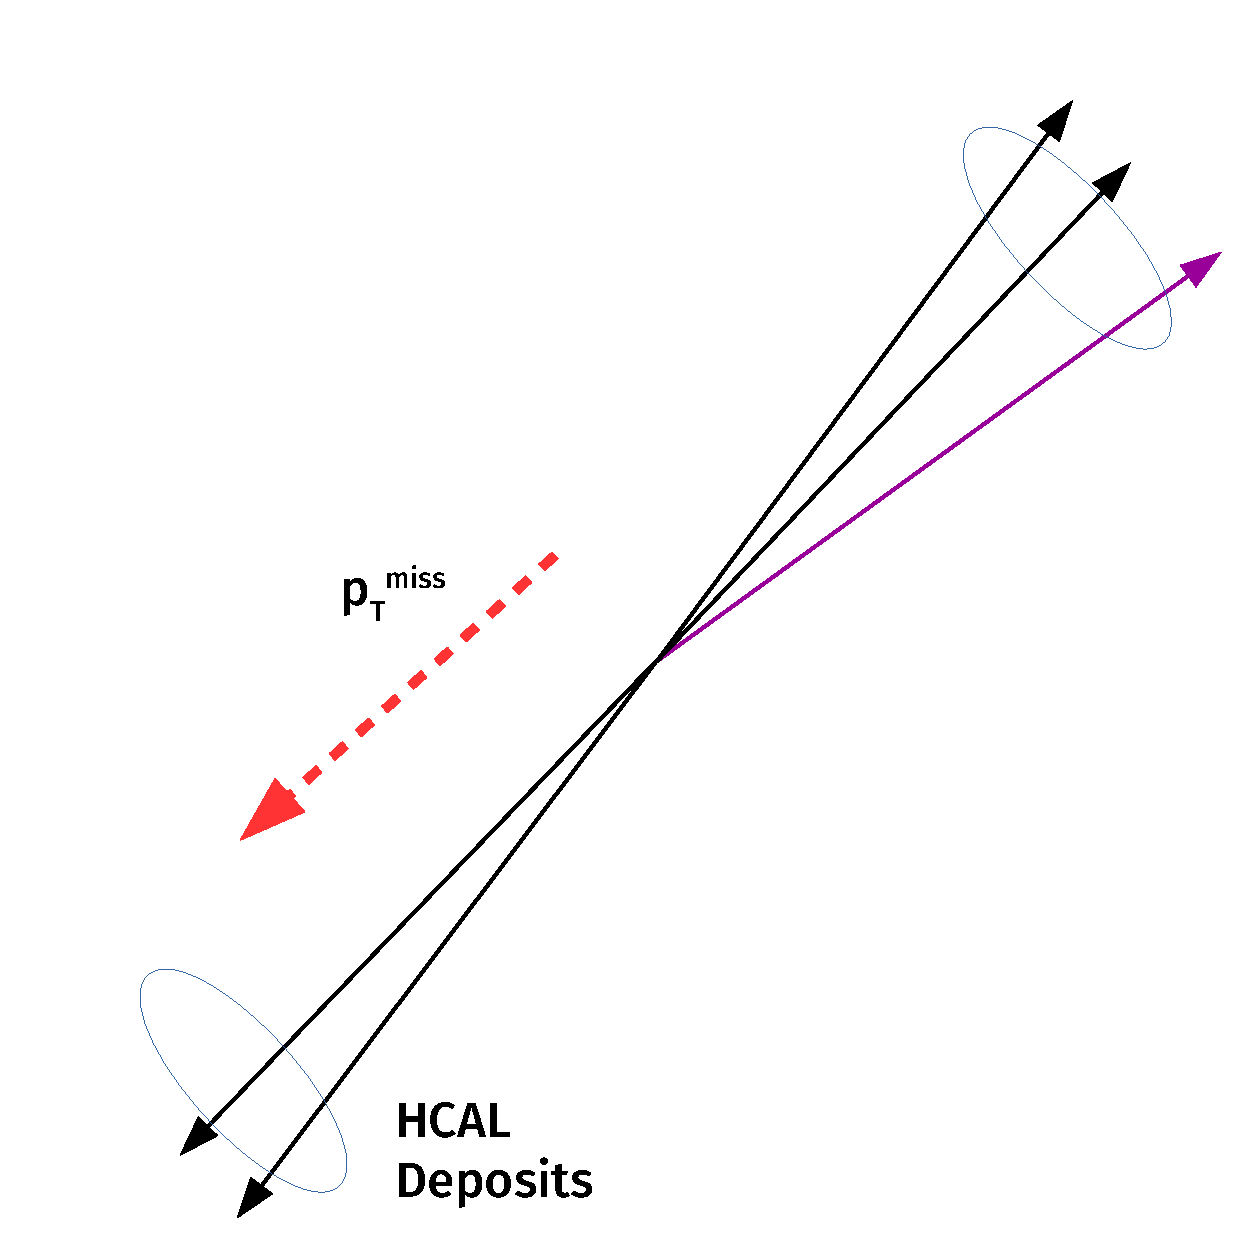
\includegraphics[width=0.49\textwidth]{figures/vbf/triggers/prefire_dijet.pdf}
            \caption{Dijet event}
        \end{subfigure}
        \begin{subfigure}[t]{0.49\textwidth}
            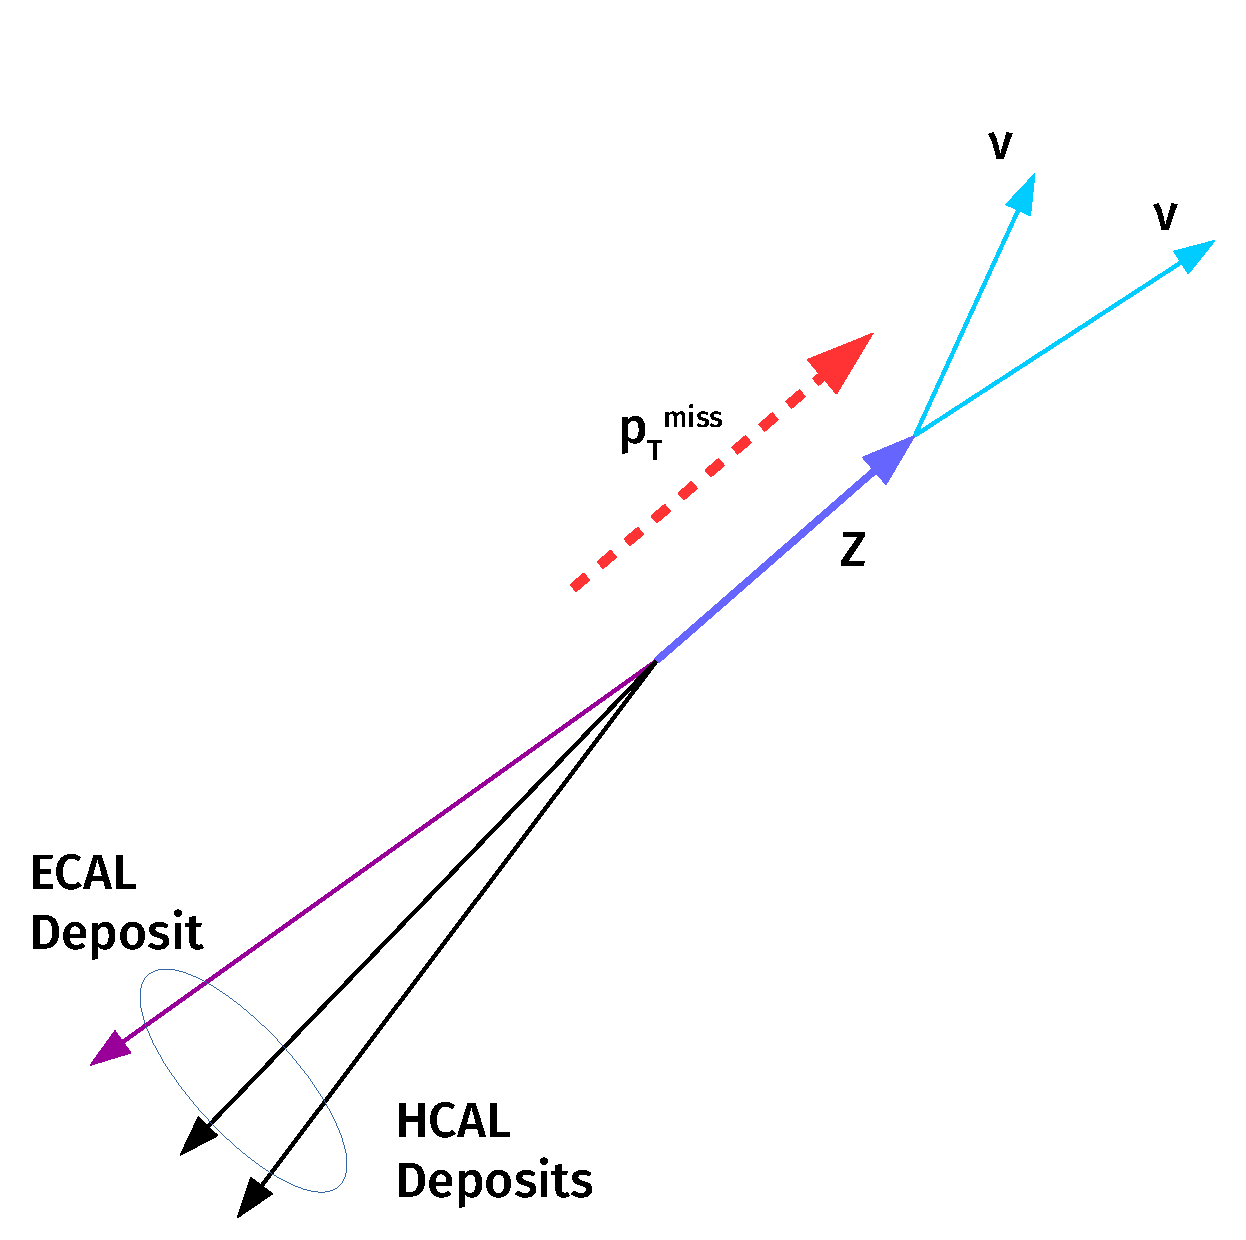
\includegraphics[width=0.49\textwidth]{figures/vbf/triggers/normal_z.pdf}
            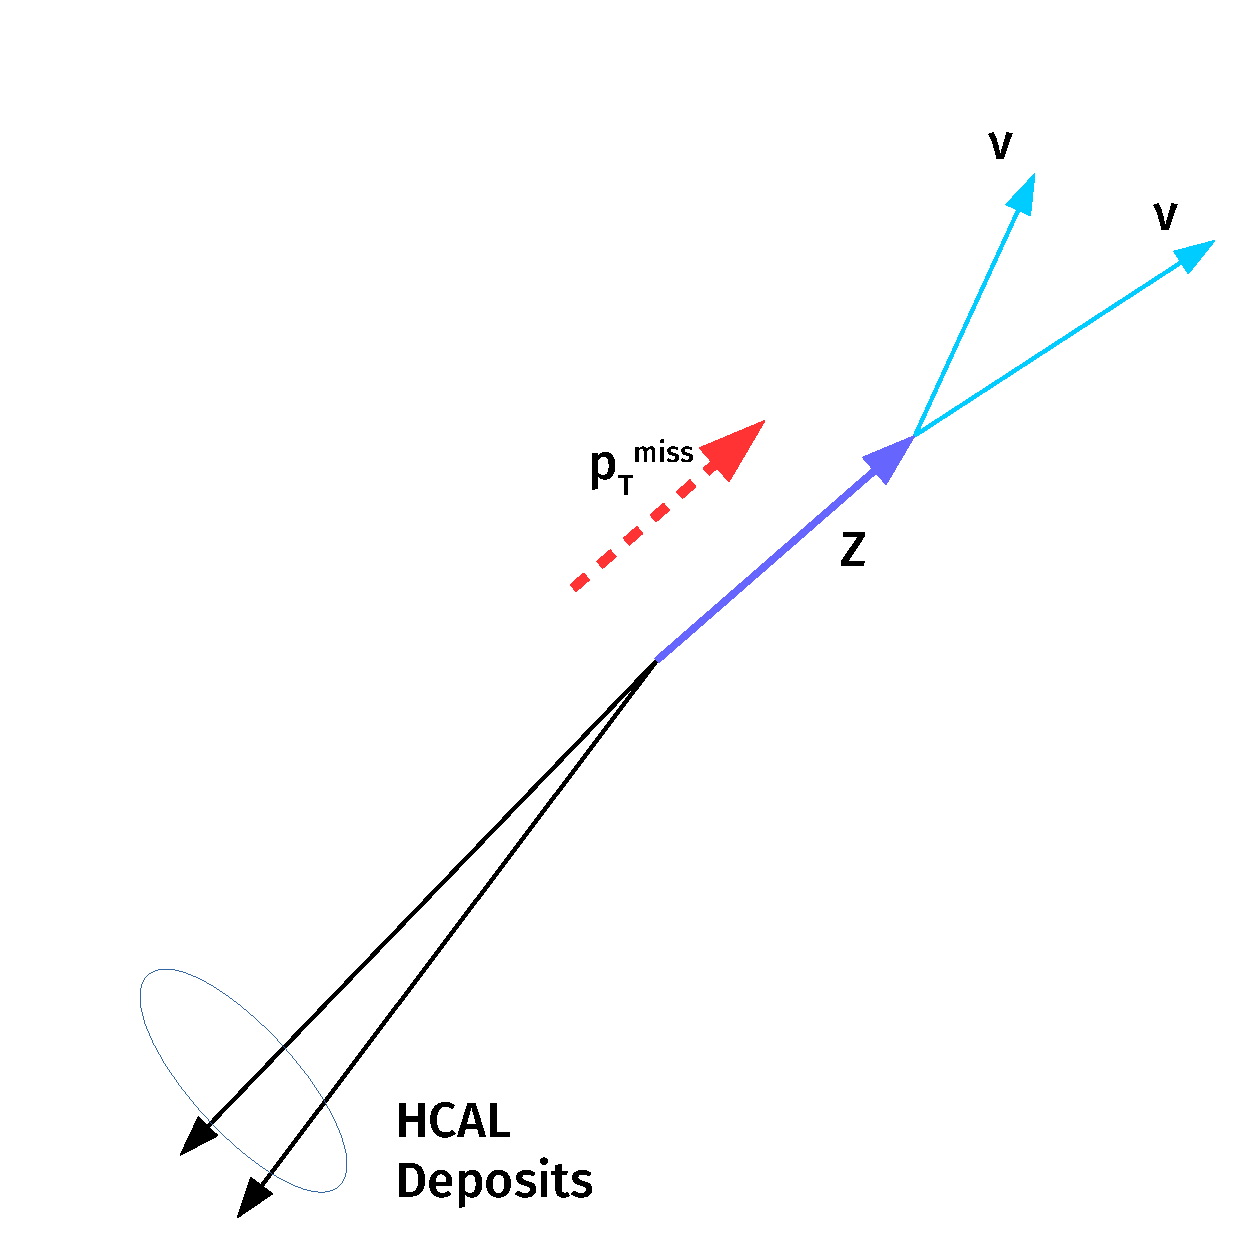
\includegraphics[width=0.49\textwidth]{figures/vbf/triggers/prefire_z.pdf}
            \caption{$Z\rightarrow\nu\nu$ event}
        \end{subfigure}
        \caption{How zero suppression in the ECAL due to pre-firing can bias certain events.
                 Subfigure (a) shows a dijet event, in which the loss of an ECAL deposit reduces the total $H_\mathrm{T}$ of the event, thereby lowering the probability of a jet-based trigger to fire.
                 Subfigure (b) shows a $Z\rightarrow\nu\nu$ event, in which the loss of an ECAL deposit reduces the total $\ptmiss$ of the event.}
        \label{fig:vbf:pre_diag}
    \end{center}
\end{figure}

The probability of at least one jet pre-firing in an event is:
\begin{equation}
    \epsilon_\text{pre-fire}^\text{event} = 1 - \prod_{j\in\text{jets}}  \left(1-\epsilon_\text{pre-fire}(\pt^j,\eta^j)\right)
\end{equation}
The $\phi$-dependence has been dropped, since it is clear from Figure~\ref{fig:vbf:pre_eff2_etaphi} that the effect can be averaged over $\phi$ once the spike is removed. 
Figure~\ref{fig:vbf:pre_eff2_pteta} shows $\epsilon_\text{pre-fire}(\pt,\eta)$ using muon-triggered and jet-triggered events.
In the former case, statistical fluctuations make the region with $\pt>250$ GeV unusable.
Fortunately, this is the region in which the trigger bias is smallest, and so we switch to the jet-triggered measurement above this threshold.
A 20\% uncertainty is assessed on the efficiency, which is derived from the difference between the SingleMuon and JetHT measurements. 

\begin{figure}[]
    \begin{center}
        \begin{subfigure}[t]{0.49\textwidth}
            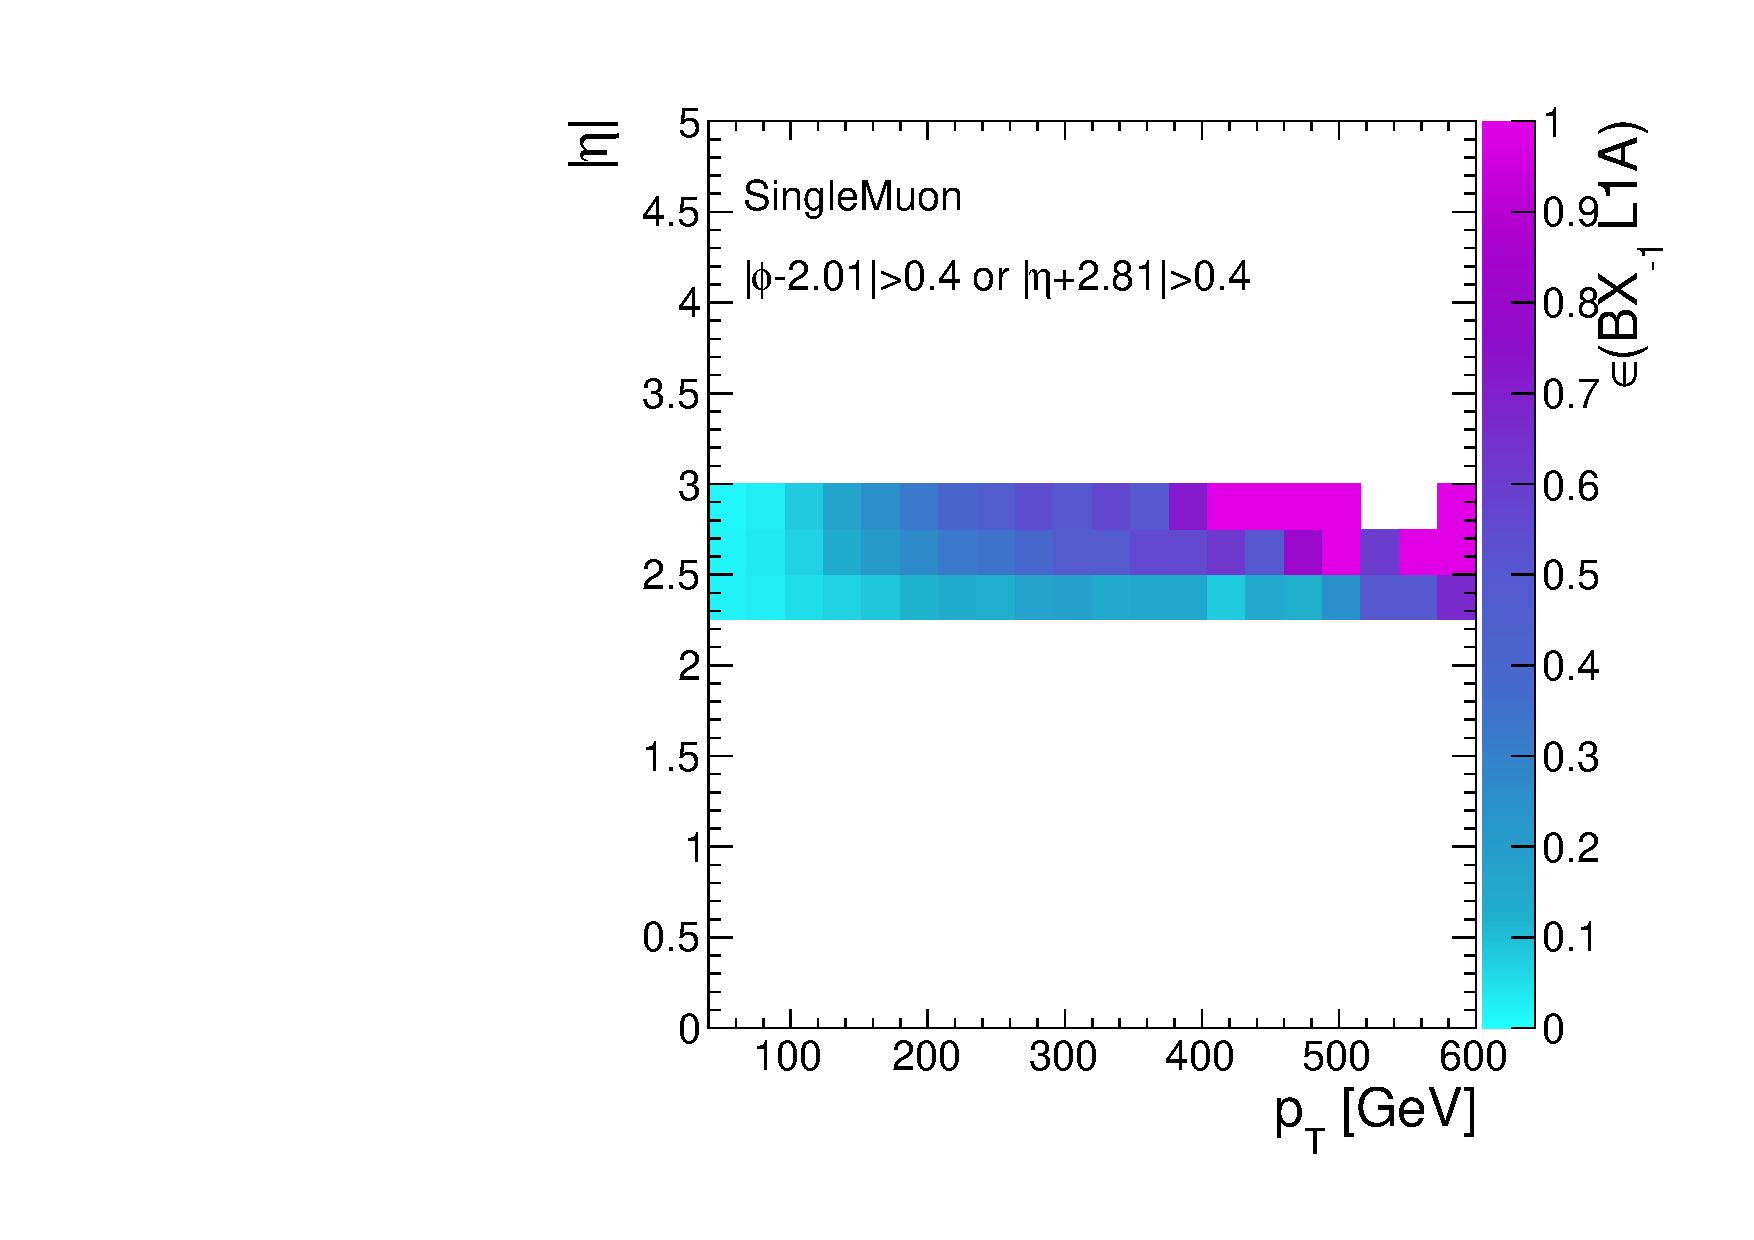
\includegraphics[width=\textwidth]{figures/vbf/triggers/SingleMuon_spike_finor_pteta_ratio.pdf}
            \caption{Muon-triggered}
        \end{subfigure}
        \begin{subfigure}[t]{0.49\textwidth}
            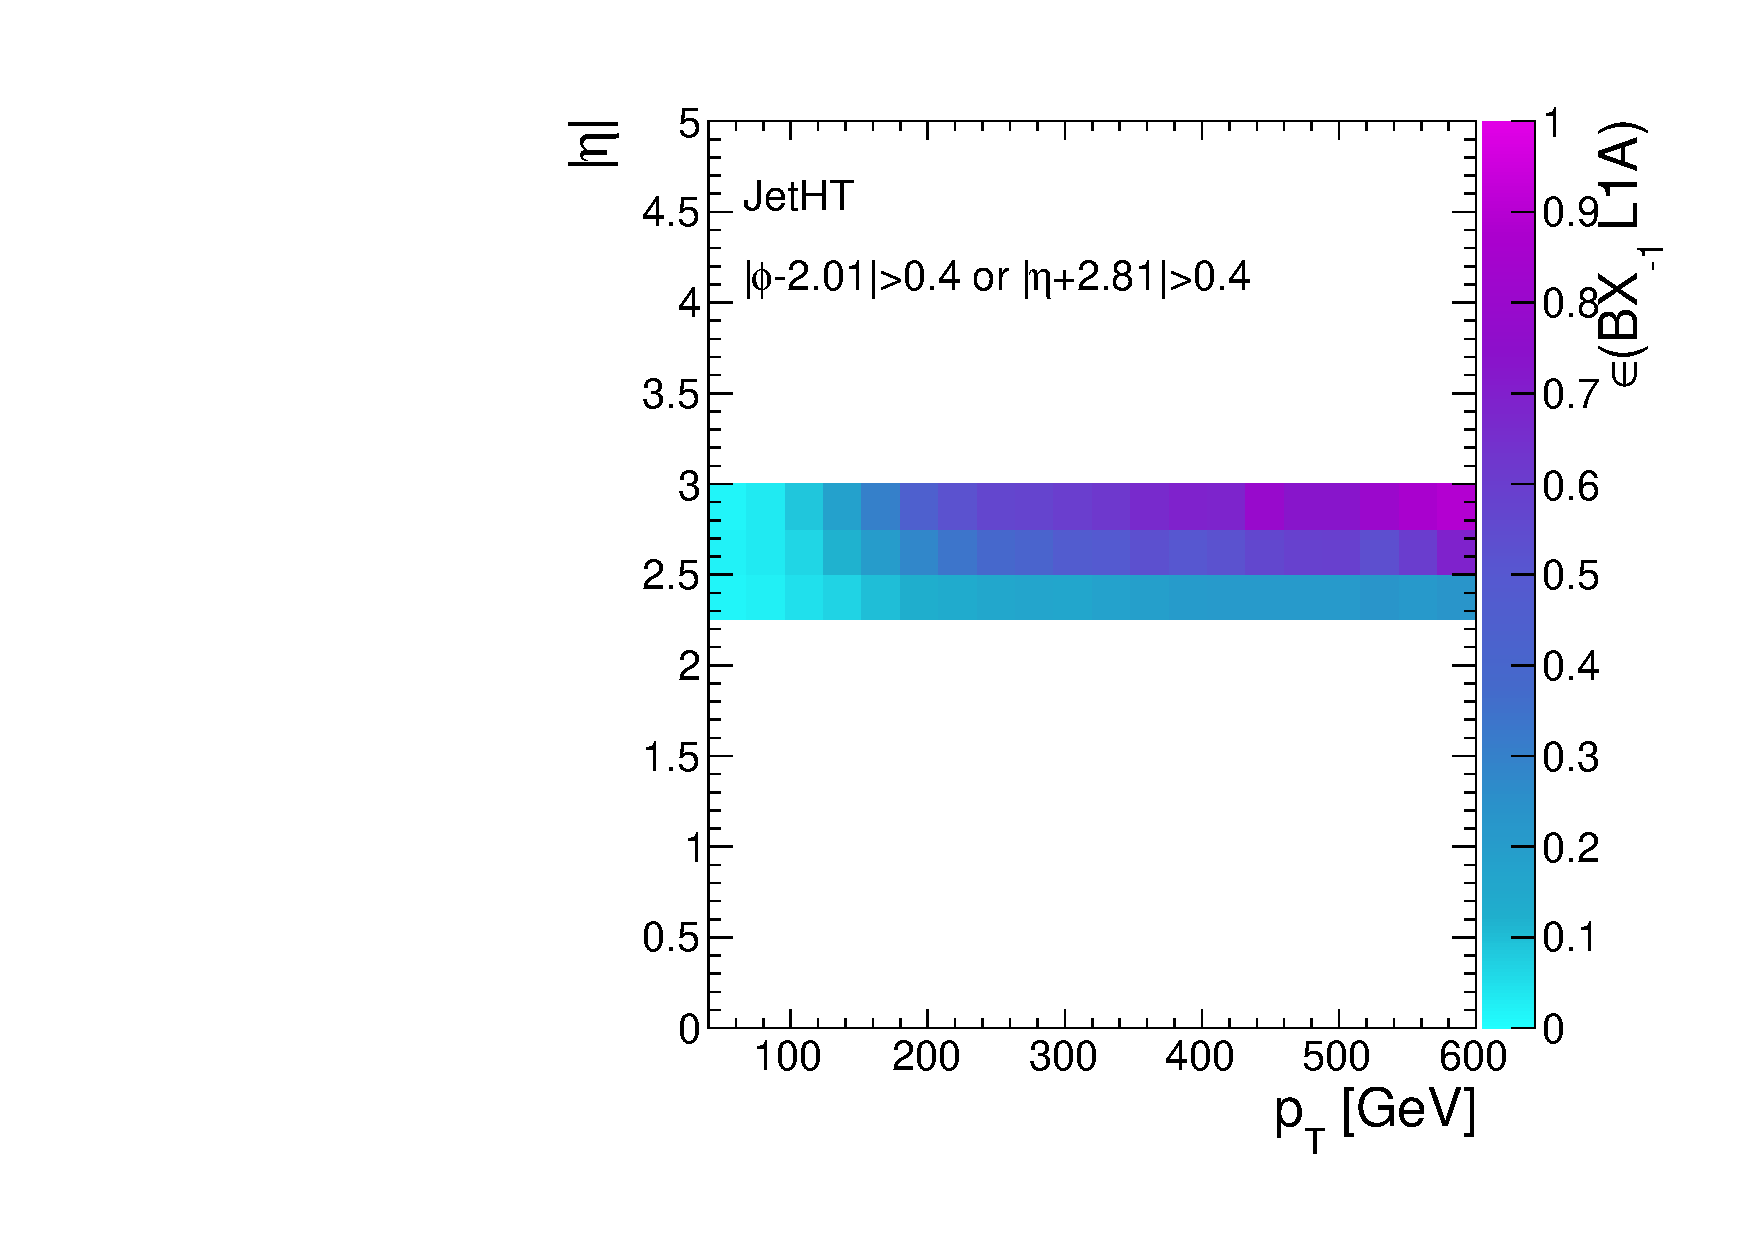
\includegraphics[width=\textwidth]{figures/vbf/triggers/JetHT_spike_finor_pteta_ratio.pdf}
            \caption{Jet-triggered}
        \end{subfigure}
        \caption{$\epsilon_\text{pre-fire}(\pt,\eta)$ with two different sets of reference triggers used to select \bx{0}.}
        \label{fig:vbf:pre_eff2_pteta}
    \end{center}
\end{figure}
